\section{Realtime Systems}

\begin{frame}
  \frametitle{Realtime Operating System}
   A real-time system is a time-bound system which has well-defined, fixed time constraints. Processing must be done within the defined constraints or the system will fail.

	\begin{center}\footnotesize{Wikipedia}\end{center}
		\begin{itemize}
			\item The correctness of the program's computations is important
			\item The time taken to perform the computation is equally important
		\end{itemize}
\end{frame}

\begin{frame}
  \frametitle{Determinism}
  The same input must always yield the same output
	\begin{itemize}
		\item In an Realtime system, the timing for event and data processing must be consistent
		\item This is trivial on single-task single-core systems
		\item On multi-tasking systems, critical tasks should be deterministic
		\item The influence of CPU sharing and external interrupts must be fully predictable
	\end{itemize}
\end{frame}

\begin{frame}
  \frametitle{Latencies}
  Time elapsed between an event and the reaction to the event
	\begin{itemize}
		\item The Worst Case Execution Time is very difficult to predict
		\item We therefore want bounds on the Worst Case Reaction Time
		\item Latencies are the main focus for Realtime Operating Systems
	\end{itemize}
	\begin{center}
		\includegraphics[width=0.9\textwidth]{slides/realtime-linux-realtime-systems/latency-basic.pdf}
	\end{center}
\end{frame}

\begin{frame}
	\frametitle{Design constraints - Throughput}
	\begin{columns}
	\begin{column}{0.35\textwidth}
	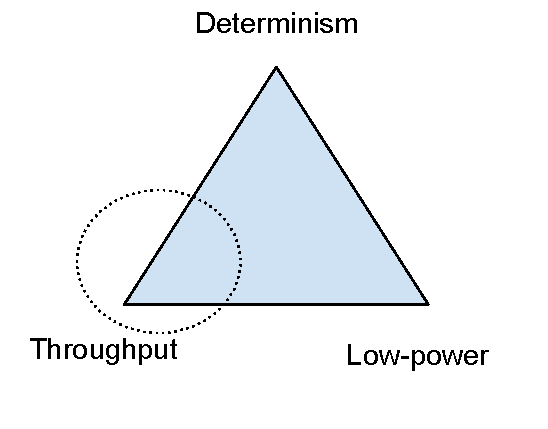
\includegraphics[width=\textwidth]{slides/realtime-linux-realtime-systems/triangle_design_throughput.pdf}
	\end{column}
		\begin{column}{0.65\textwidth}
			\begin{itemize}
				\item Optimize most-likely scenario
				\item Might have a fast path and a slow path
				\item Use Hardware Offloading and caches
				\item Use Branch-Prediction and Speculative execution
				\item Latencies are acceptable for cold-start
				\item Most modern hardware implement such features
			\end{itemize}
		\end{column}
	\end{columns}
\end{frame}

\begin{frame}
	\frametitle{Design constraints - Low Power}
	\begin{columns}
	\begin{column}{0.35\textwidth}
	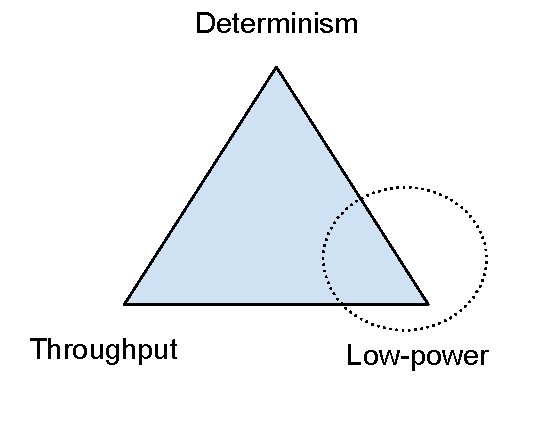
\includegraphics[width=\textwidth]{slides/realtime-linux-realtime-systems/triangle_design_power.pdf}
	\end{column}
		\begin{column}{0.65\textwidth}
			\begin{itemize}
				\item Oportunistic sleeping modes
				\item Dynamic Frequency Scaling
				\item Only go fast when required
				\item Long wakeup latencies
				\item Power-Management firmwares can preempt the whole system
			\end{itemize}
		\end{column}
	\end{columns}
\end{frame}

\begin{frame}
	\frametitle{Design constraints - Determinism}
	\begin{columns}
	\begin{column}{0.35\textwidth}
	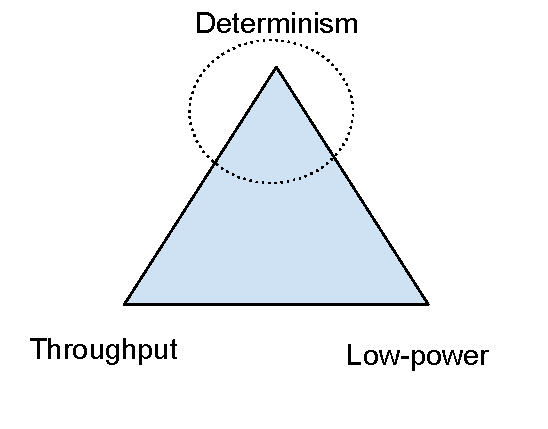
\includegraphics[width=\textwidth]{slides/realtime-linux-realtime-systems/triangle_design_determinism.pdf}
	\end{column}
		\begin{column}{0.65\textwidth}
			\begin{itemize}
				\item Avoid unpredictable effects
				\item Caches, Hardware Offload are hard to predict
				\item Avoid sleeping too deep, to wakeup fast
				\item Make the system fully preemptible
				\item Try to keep control over every aspect of the system
			\end{itemize}
		\end{column}
	\end{columns}
\end{frame}

\begin{frame}
	\frametitle{Security Features and Fixes}
	\begin{itemize}
		\item Hardware security flaws are discovered quite often
		\item Spectre, Meltdown, Foreshadow, Rowhammer
		\item Some can only be mitigated through software fixes...
		\item ... that can introduce some latencies
		\item In other cases, security features are actually beneficial for Realtime
		\item To mitigate timing-based attacks, making the system predictable is crucial
		\item \textbf{core scheduling} is also a good example, to deal with Hyperthreading issues
	\end{itemize}
\end{frame}

\begin{frame}
  \frametitle{Multi-tasking}
	\begin{itemize}
		\item Modern OSes are designed to be multi-task
		\item The CPU time is shared between applications
		\item The Scheduler decides who runs at any given time
		\item The scheduler is invoked at several occasions :
			\begin{itemize}
				\item When an application waits for external data or events
				\item When external data or events needs to be processed
				\item Periodically, at every \textbf{System Tick} (between 300Hz and 1KHz)
				\item Tickless systems are throughput oriented, but can also be useful for RT
			\end{itemize}
		\item Switching between tasks is called \textbf{context switching}
	\end{itemize}
\end{frame}

\begin{frame}
	\frametitle{Preemption}
	\begin{itemize}
		\item Ability to stop whatever the CPU is running to run another task
		\item Useful for general-purpose OS, to share execution time
		\item Critical for an RTOS, to run critical tasks
		\item Any task should be preemptible, both in userspace and kernelspace
	\end{itemize}
\end{frame}

\begin{frame}
  \frametitle{Understanding preemption (1)}
  \begin{itemize}
  \item Most multi-tasking OSses are preemptive operating systems, including Linux
  \item When a task runs in user space mode and gets interrupted by an
    interruption, if the interrupt handler wakes up another task, this
    task can be scheduled as soon as we return from the interrupt
    handler.
  \end{itemize}
  \begin{center}
    \includegraphics[width=0.9\textwidth]{slides/realtime-linux-realtime-systems/userspace-preemption.pdf}
  \end{center}
\end{frame}

\begin{frame}
  \frametitle{Understanding preemption (2)}
  \begin{itemize}
  \item However, when the interrupt comes while the task is executing
    a system call, this system call has to finish before another task
    can be scheduled.
  \item By default, the Linux kernel does not do kernel preemption.
  \item This means that the time before which the scheduler will be
    called to schedule another task is unbounded.
  \end{itemize}
  \begin{center}
    \includegraphics[width=\textwidth]{slides/realtime-linux-realtime-systems/kernel-preemption.pdf}
  \end{center}
\end{frame}


\begin{frame}
  \frametitle{Interrupts and events}
	\begin{itemize}
		\item Hardware interrupts are a common source of latencies
		\item Interrupts run in a dedicated context
		\item Other interrupts are disabled while the interrupt handler runs
		\item Non-important interrupts can preempt critical tasks
	\end{itemize}
	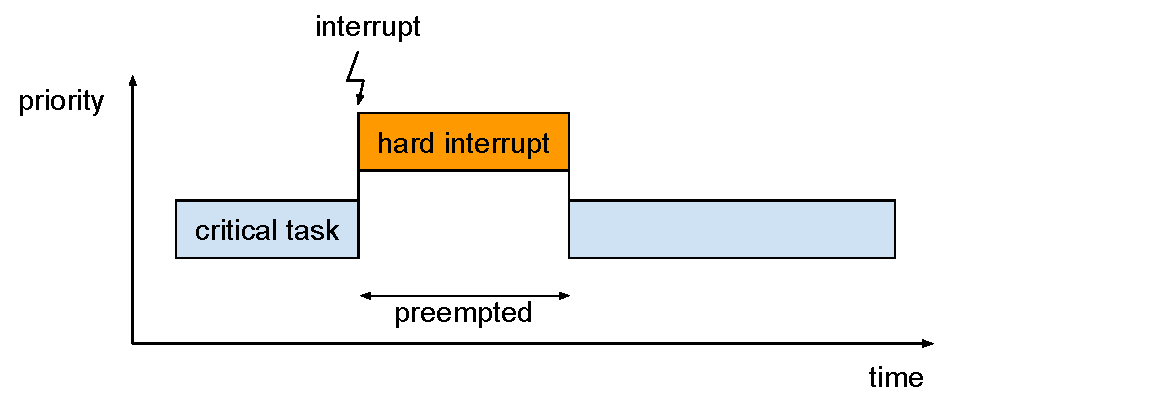
\includegraphics[height=0.5\textheight]{slides/realtime-linux-realtime-systems/irq_preemption.pdf}
	% irq_preemption.pdf
\end{frame}

\begin{frame}
  \frametitle{Scheduling and proritizing}
	\begin{itemize}
		\item The Scheduler is a key component in guaranteeing RT behaviour
		\item There exist realtime and non-realtime scheduling algorithms
		\item Most realtime OSes rely on task prioritization
		\item Tasks with the same priority can be handled in a FIFO or Round-Robin manner
	\end{itemize}
\end{frame}

\begin{frame}
  \frametitle{Locking}
	\begin{itemize}
		\item Multitasking implies concurrent accesses to resources
		\item Critical resources must be protected by a dedicated mechanism
		\item Mutexes and semaphores help synchronise (or serialize) accesses
		\item This needs to be looked at closely in RT context
		\item A low-priority task migh hold a lock, blocking a high-priority task
	\end{itemize}
	\begin{itemize}
		\item \textbf{mutex} : Two states (taken, free). The task that has taken the mutex is the \textbf{owner}
		\item \textbf{semaphore} : Shared variable that is incremented by multiple users.
	\end{itemize}
\end{frame}

\begin{frame}
	\frametitle{Lock Families}
		\begin{center}\textbf{Semaphores}\end{center}
		\begin{itemize}
			\item Semaphores rely on a \textbf{counter} that is positive or null
			\item A task trying to access the critical section decrements a counter
			\item A task is blocked if the counter can't be decremented
			\item Multiple tasks can be in a critical section, hence there's no single owner
		\end{itemize}
		\begin{center}\textbf{Mutexes}\end{center}
		\begin{itemize}
			\item \textbf{Mut}ually \textbf{ex}clusive
			\item Have two states : Taken, Free
			\item The task that has taken the mutex is the \textbf{owner}
			\item Other tasks wait for the mutex to be free before taking it
			\item A Mutex is a semaphore with a counter that can only be incremented once
		\end{itemize}


\end{frame}

\begin{frame}
  \frametitle{Priority inversion}
	\begin{itemize}
		\item Priority inversion arises when strict priority-based scheduling interfers with locking
		\item It creates a scenario where a critical task is
		      prevented from running by a lower priority task
	\end{itemize}
\end{frame}

\begin{frame}
  \frametitle{Priority inversion}
	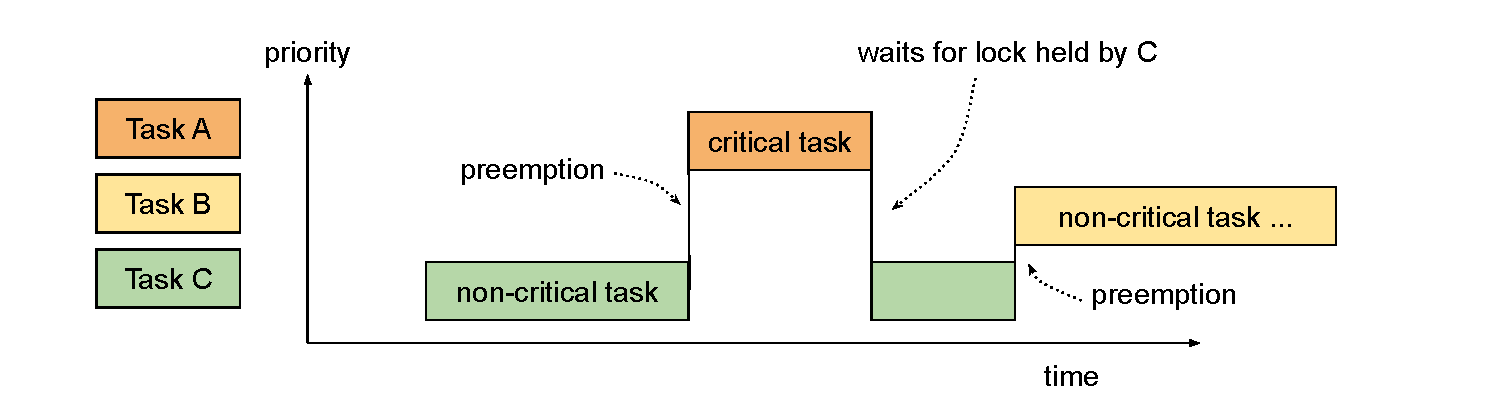
\includegraphics[height=0.5\textheight]{slides/realtime-linux-realtime-systems/priority_inversion.pdf}
	% priority_inversion.pdf
	\begin{itemize}
		\item Task A (high priority) needs to access a lock, hold by task C (low priority)
		\item The scheduler runs task C so that it can release the lock
		\item Task B has a higher priority than C, but lower than A, preempts task C
	\end{itemize}
\end{frame}

\begin{frame}
  \frametitle{Priority Inheritance}
	\begin{itemize}
		\item The solution for the Priority Inversion issue is \textbf{priority inheritance}
		\item The scheduler detects that task C holds a lock needed by task A
		\item Task C's priority is boosted to A's priority until it releases the lock
		\item Task B can no longer preempt task C !
	\end{itemize}
	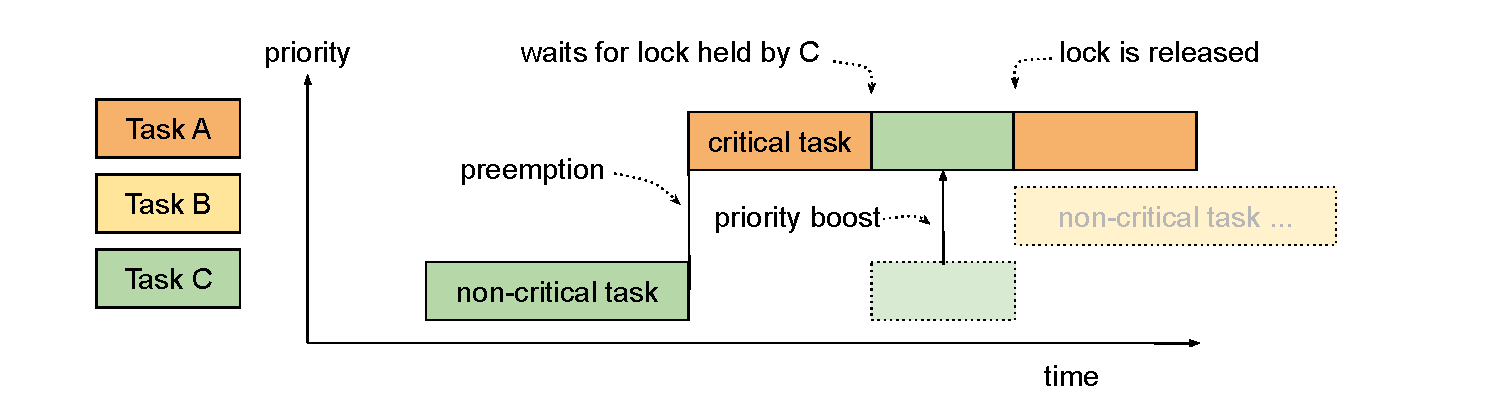
\includegraphics[height=0.5\textheight]{slides/realtime-linux-realtime-systems/priority_inheritance.pdf}
	%priority_inheritance.pdf
\end{frame}

\begin{frame}
	\frametitle{Priority Inheritance (2)}
	\begin{itemize}
		\item \textbf{P}riority \textbf{I}nheritance (PI) only works with Mutexes
		\item Semaphores don't have owners, so we can't apply this mechanism
		\item Another way to prevent Priority Inversion is by careful design
		\item Limit critical section accesses only to tasks with the same priority
		\item PI support exists for \code{pthread_mutex_t} in Linux
	\end{itemize}
\end{frame}
